
%(BEGIN_QUESTION)
% Copyright 2010, Tony R. Kuphaldt, released under the Creative Commons Attribution License (v 1.0)
% This means you may do almost anything with this work of mine, so long as you give me proper credit

Suppose a Siemens 545 PLC has the following input bit states:

\begin{itemize}
\item{} {\tt X1} = 0
\item{} {\tt X2} = 1
\item{} {\tt X3} = 0
\end{itemize}

Sketch color highlighting for the contacts and coils in the PLC's program given these bit statuses, also determining the status of output bit {\tt Y1}:

$$\includegraphics[width=15.5cm]{i04688x01.eps}$$

\vskip 20pt \vbox{\hrule \hbox{\strut \vrule{} {\bf Suggestions for Socratic discussion} \vrule} \hrule}

\begin{itemize}
\item{} PLC training expert Ron Beaufort teaches students to think of a ``normally-open'' PLC program contact instruction as a command to the PLC's processor to {\it ``Go look for a 1''}.  Conversely, he teaches students to think of a ``normally-closed'' instruction as a command to {\it ``Go look for a 0''}.  Explain what Mr. Beaufort means by these phrases, and how this wisdom relates to this particular problem.  Incidentally, Mr. Beaufort's excellent instructional videos (available freely on YouTube) are quite valuable to watch!
\item{} Identify the significance of the labels ``X'' and ``Y'' for this PLC's bits.  What do you suppose ``X'' signifies?  What do you suppose ``Y'' signifies?
\item{} Sketch a logic gate diagram implementing the same function as this PLC program.
\end{itemize}

\underbar{file i04688}
%(END_QUESTION)





%(BEGIN_ANSWER)

$$\includegraphics[width=15.5cm]{i04688x02.eps}$$

\begin{itemize}
\item{} {\tt Y1} = 1
\end{itemize}

%(END_ANSWER)





%(BEGIN_NOTES)


%INDEX% PLC, relating I/O status to virtual elements 

%(END_NOTES)


